%% LyX 2.3.2-2 created this file.  For more info, see http://www.lyx.org/.
%% Do not edit unless you really know what you are doing.
\documentclass[czech,english,american]{beamer}
\usepackage[T1]{fontenc}
\usepackage[utf8]{inputenc}
\setcounter{secnumdepth}{3}
\setcounter{tocdepth}{3}
\usepackage{amsmath}
\usepackage{amssymb}
\usepackage{graphicx}

\makeatletter

%%%%%%%%%%%%%%%%%%%%%%%%%%%%%% LyX specific LaTeX commands.
%% A simple dot to overcome graphicx limitations
\newcommand{\lyxdot}{.}


%%%%%%%%%%%%%%%%%%%%%%%%%%%%%% Textclass specific LaTeX commands.
% this default might be overridden by plain title style
\newcommand\makebeamertitle{\frame{\maketitle}}%
% (ERT) argument for the TOC
\AtBeginDocument{%
  \let\origtableofcontents=\tableofcontents
  \def\tableofcontents{\@ifnextchar[{\origtableofcontents}{\gobbletableofcontents}}
  \def\gobbletableofcontents#1{\origtableofcontents}
}

%%%%%%%%%%%%%%%%%%%%%%%%%%%%%% User specified LaTeX commands.
\usetheme{Szeged}
\usecolortheme{beaver}
\title
{Discrete random walks with memory: Models and applications}
%\subtitle{Teze dizertační práce}
%\logo{\includegraphics[height=1.3cm]{../../../fjfi.pdf}}
\institute[\selectlanguage{czech}%
UTIA\selectlanguage{czech}%
]{Institute of Information Theory and Automation, AS CR Prague}
\date{16.9.2019}
\author[\selectlanguage{czech}%
Ing. Tomáš Kouřim\selectlanguage{czech}%
]{Ing. Tomáš~Kouřim \and }
\newcommand{\nologo}{\setbeamertemplate{logo}{}} % command to set the logo to nothing
\usepackage[czech]{babel}
\setbeamercovered{transparent}

\makeatother

\usepackage{babel}
\begin{document}
\title{\selectlanguage{english}%
Discrete random walks with memory: Models and applications}
\makebeamertitle

\begin{frame}{Outline}

\begin{enumerate}
\item<1-> {\Large{}Prepare mathematical model}\bigskip{}
\item<2-> {\Large{}Describe its properties}\bigskip{}
\item<3-> {\Large{}Apply it on data}
\end{enumerate}
\end{frame}
%
\begin{frame}{Random walk}

\selectlanguage{english}%
\begin{definition}
A man starts from a point $O$ and walks $l$ yards in a straight
line; he then turns through any angle whatever and walks another $l$
yards in a second straight line. He repeats this process $n$ times.
I require the probability that after these $n$ stretches he is at
a distance between $r$ and $r+\delta r$ from his starting point,
$O.$


{\footnotesize{}\medskip{}
}\emph{\footnotesize{}{[}Karl Pearson: The problem of the random walk.
(1905){]}}{\footnotesize\par}

\end{definition}

\begin{description}
\item <2-> Where is the ``Drunken sailor''?
\end{description}


\end{frame}
%
\begin{frame}{Random walk}

\begin{definition}
Let${\{X_{k}\}}_{k=1}^{\infty}$be a sequence of independent, identically
distributed discrete random variables. For each positive integer $n$,
let $S_{n}$ denote the sum $X_{1}+X_{2}+\cdot\cdot\cdot+X_{n}$,
with $S_{0}=0$. The sequence $\{{S_{n}}\}{}_{n=1}^{\infty}$ is called
a random walk. If the common range of the $X_{k}$’s is $\mathbb{R}_{m}$,
then ${\{S_{n}\}}$ is a random walk in $\mathbb{R}_{m}$.

\end{definition}


{\footnotesize{}\medskip{}
}{\footnotesize\par}

For $X_{k}\sim B(p=\frac{1}{2})$ it is called the standard random
walk.
\end{frame}
%
\begin{frame}{Random walk properties}
\begin{itemize}
\item Discrete random process
\item $n-$dimensional, on a matrix, graph, finite or infinite set
\item Self avoiding, reinforced
\item Brownian motion, polymer creation, games simulation, sports simulation
\end{itemize}
\end{frame}
%

\begin{frame}{Random walk with memory}


\begin{itemize}
\item Based on standard random walk (Bernoulli distribution with $p=0.5$,
discrete time).
\item Constant total step size:
\[
l_{i}^{+}+l_{i}^{-}=2\ \forall i\in\mathbb{N}.
\]
\item At the beginning the step sizes are equal ($l_{1}^{+}=l_{1}^{-}=1$)
and further for $t>1$ evolve using a memory parameter $\lambda\in(0,\,1)$:
\[
X_{t-1}=1\rightarrow\begin{cases}
l_{t}^{+}=\lambda l_{t-1}^{+}\\
l_{t}^{-}=2-\lambda l_{t-1}^{+}
\end{cases}X_{t-1}=-1\rightarrow\begin{cases}
l_{t}^{+}=2-\lambda l_{t-1}^{-}\\
l_{t}^{-}=\lambda l_{t-1}^{-}
\end{cases}
\]
\item {\footnotesize{}Loïc Turban. }\emph{\footnotesize{}On a random walk
with memory and its relation with markovian processes. }{\footnotesize{}Journal
of Physics A: Mathematical\newline and Theoretical (2010).}{\footnotesize\par}
\end{itemize}
\end{frame}
%
\begin{frame}{Random walk with varying transition probability}
\begin{itemize}
\item Based on standard random walk (Bernoulli distribution with $p=0.5$,
discrete time).
\item Step size remains constant, transition probability changes
\item First step realized according to starting probability $p_{0}$ which
then for $t>1$ evolve using a memory parameter $\lambda\in(0,\,1)$:
\[
X_{t}=1\rightarrow p_{t}=\lambda p_{t-1}
\]
\[
X_{t}=-1\rightarrow p_{t}=1-\lambda(1-p_{t-1})
\]
\end{itemize}
\end{frame}
%
\begin{frame}{Example - RW evolution}

\includegraphics[width=1\textwidth]{examples_p0=0\lyxdot 50}
\end{frame}
%
\begin{frame}{Example - Expected position of the walker}

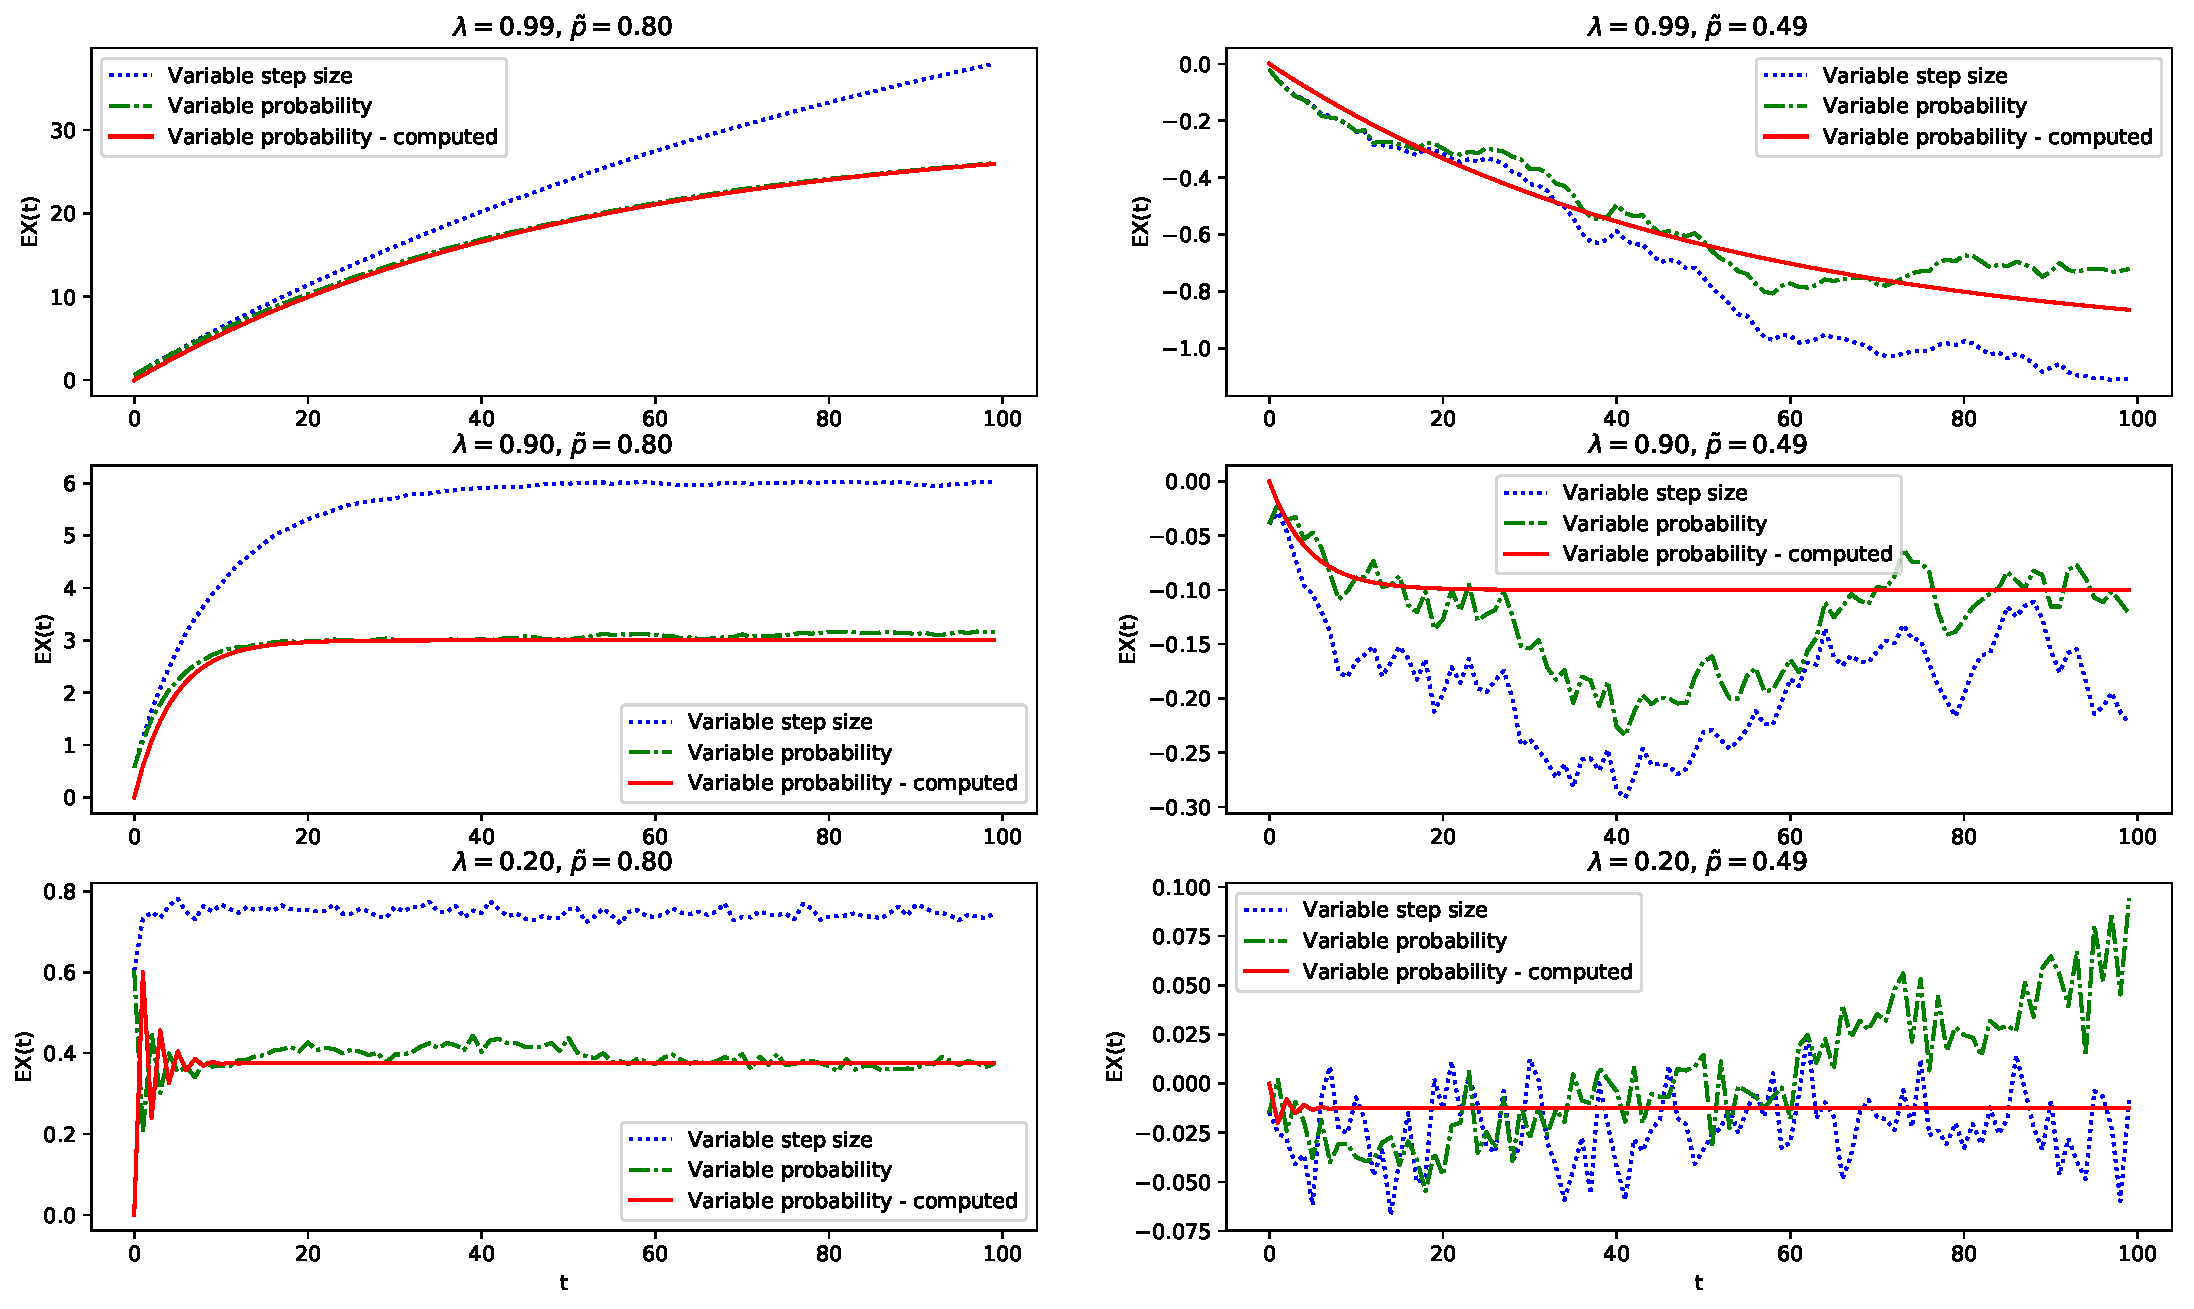
\includegraphics[width=1\textwidth]{EXt}
\end{frame}
%
\begin{frame}{Example - Expected transition probability}

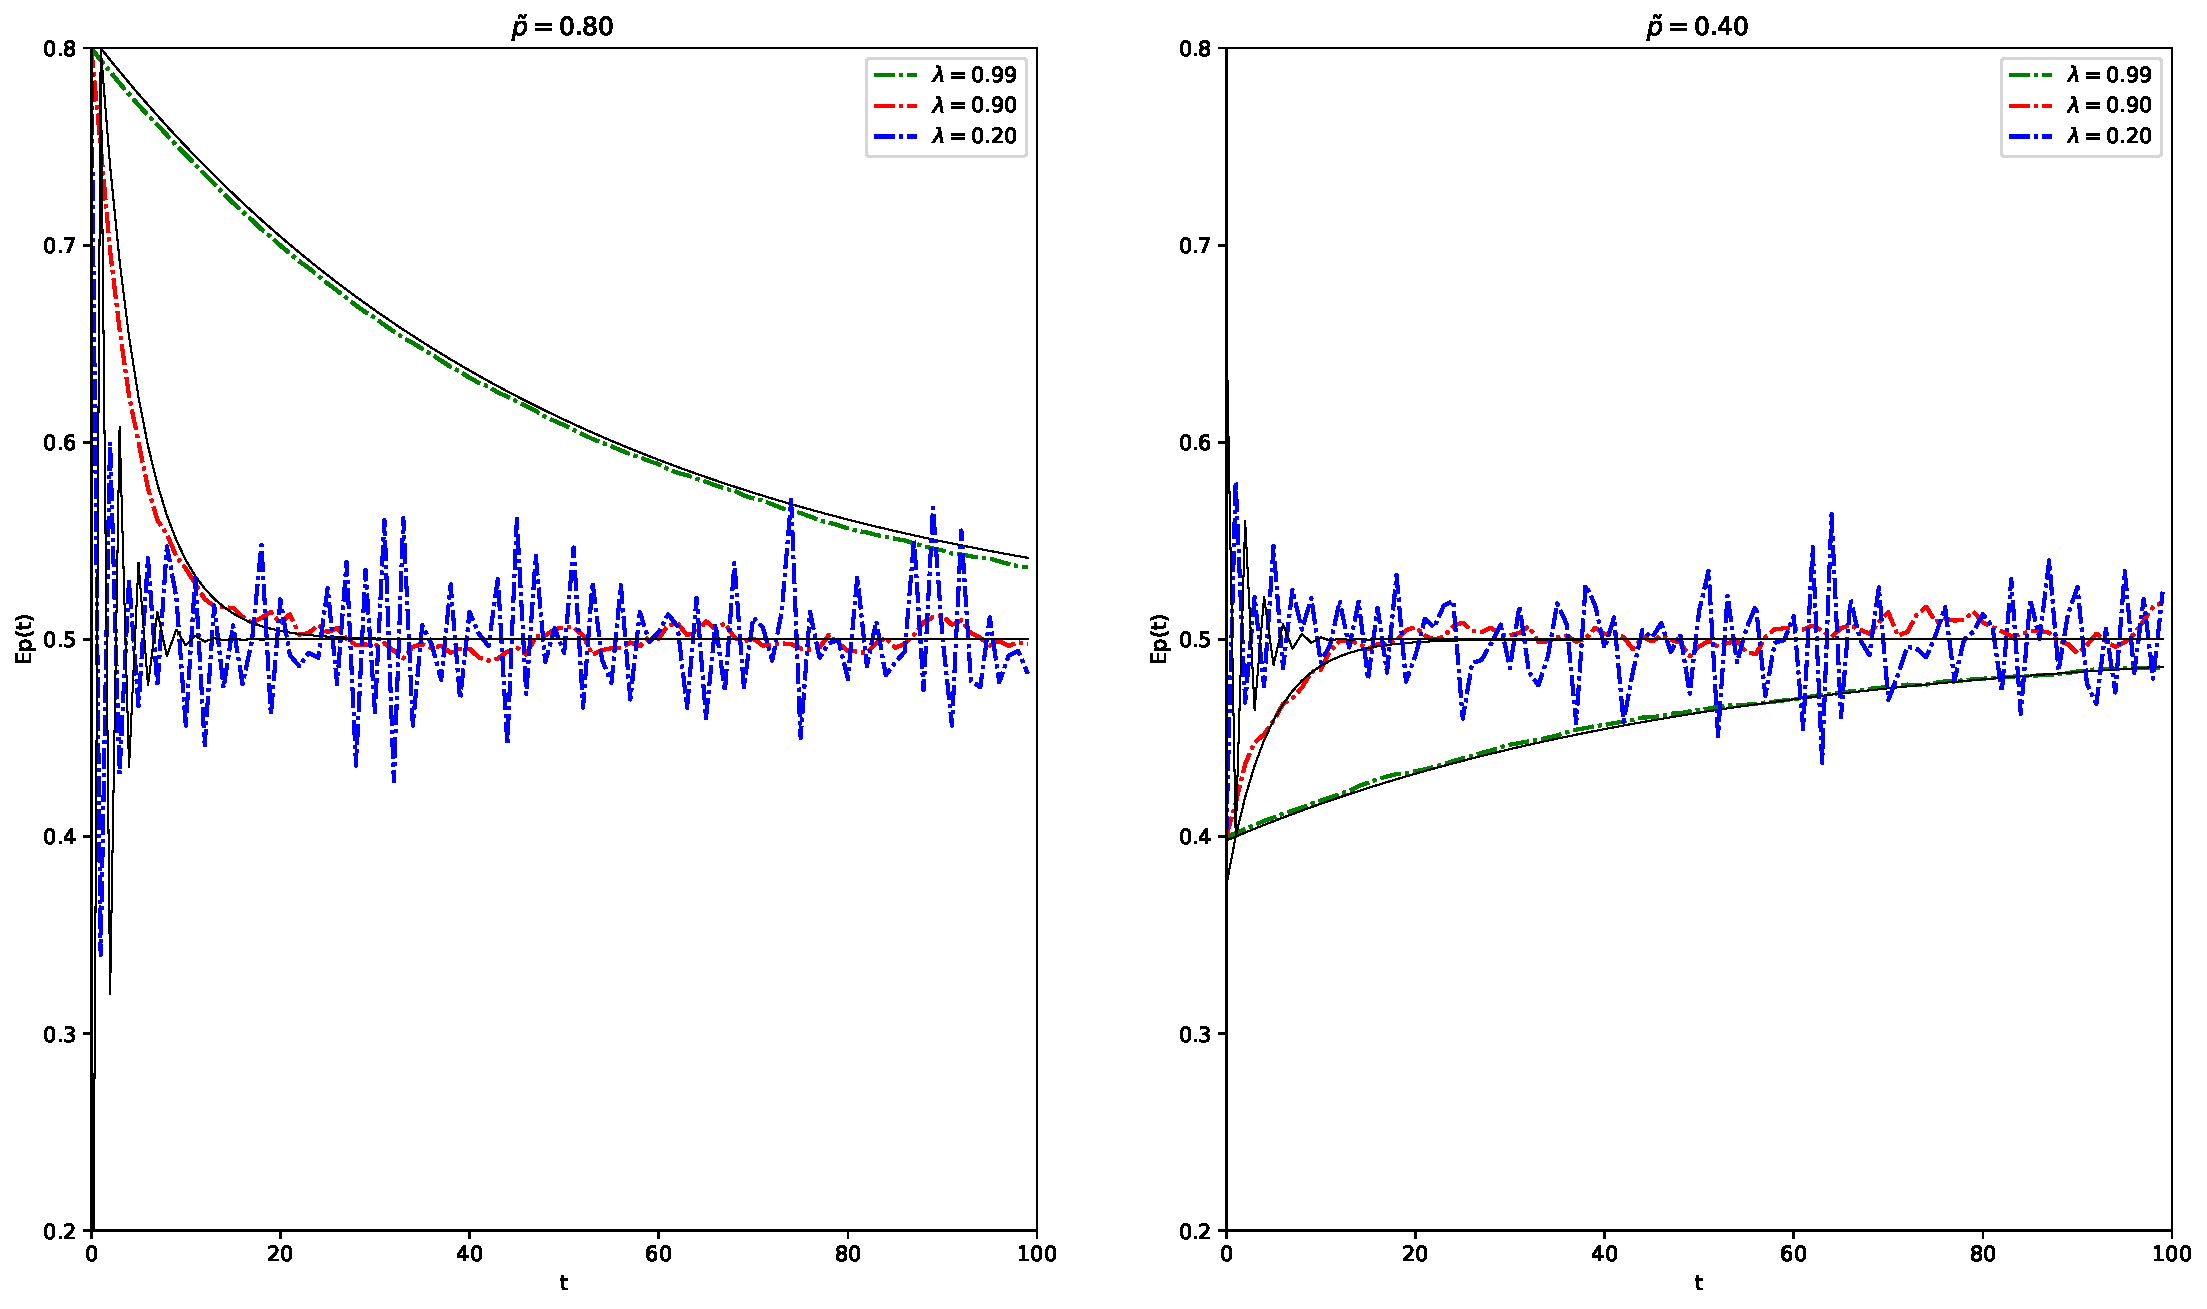
\includegraphics[width=1\textwidth]{Ept}
\end{frame}
%
\begin{frame}{Example - Transition probability variance}

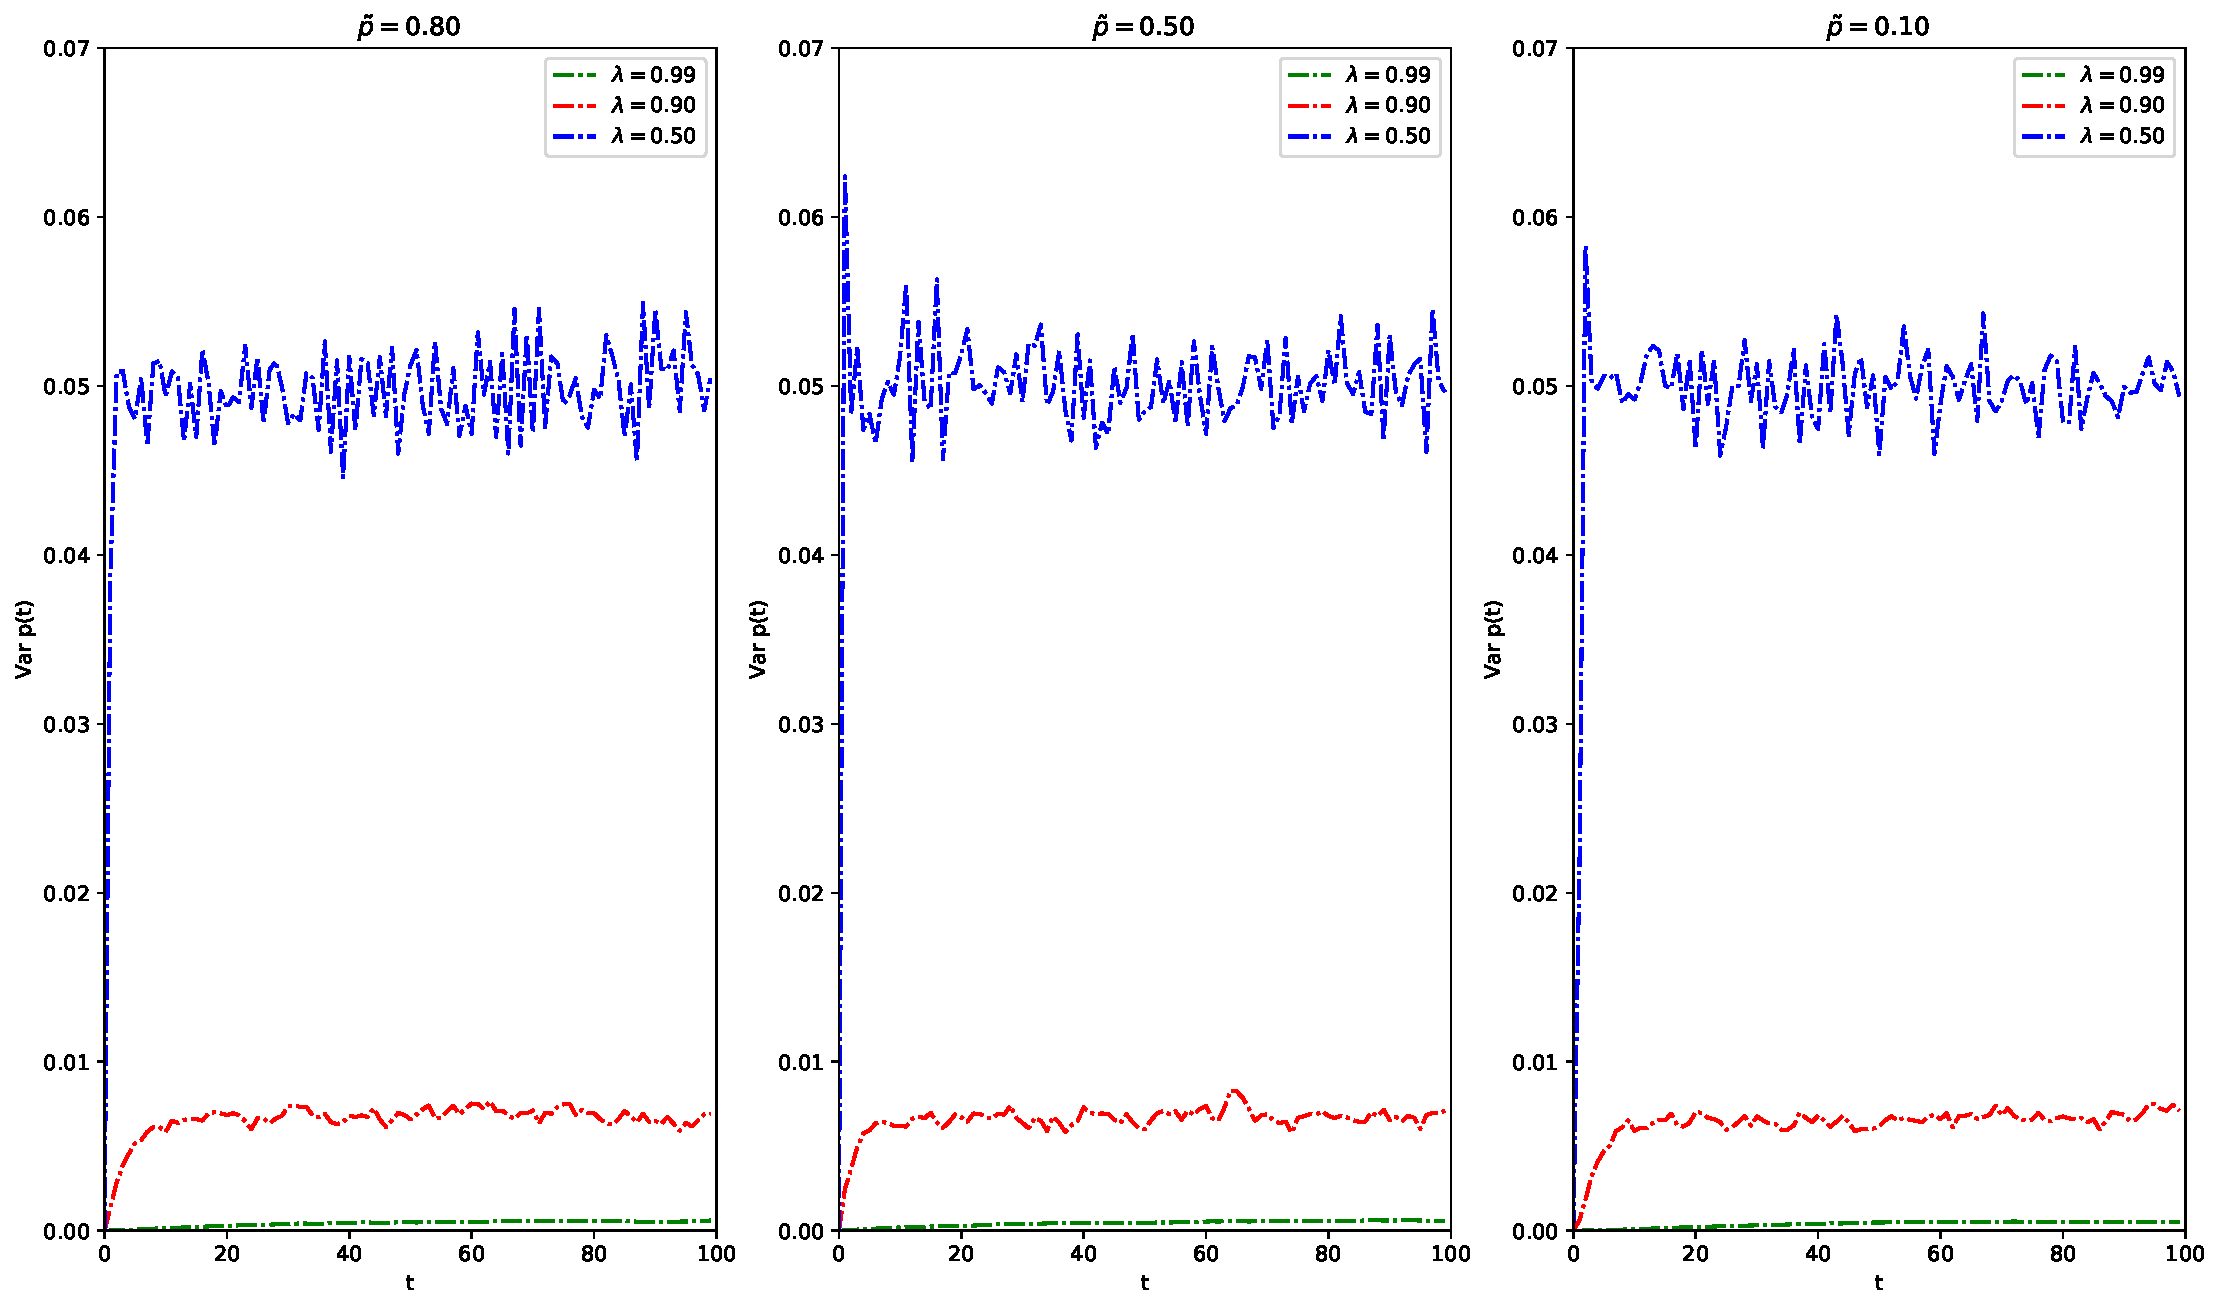
\includegraphics[width=1\textwidth]{Varpt}
\end{frame}
%
\begin{frame}{Example - Walker's position variance}

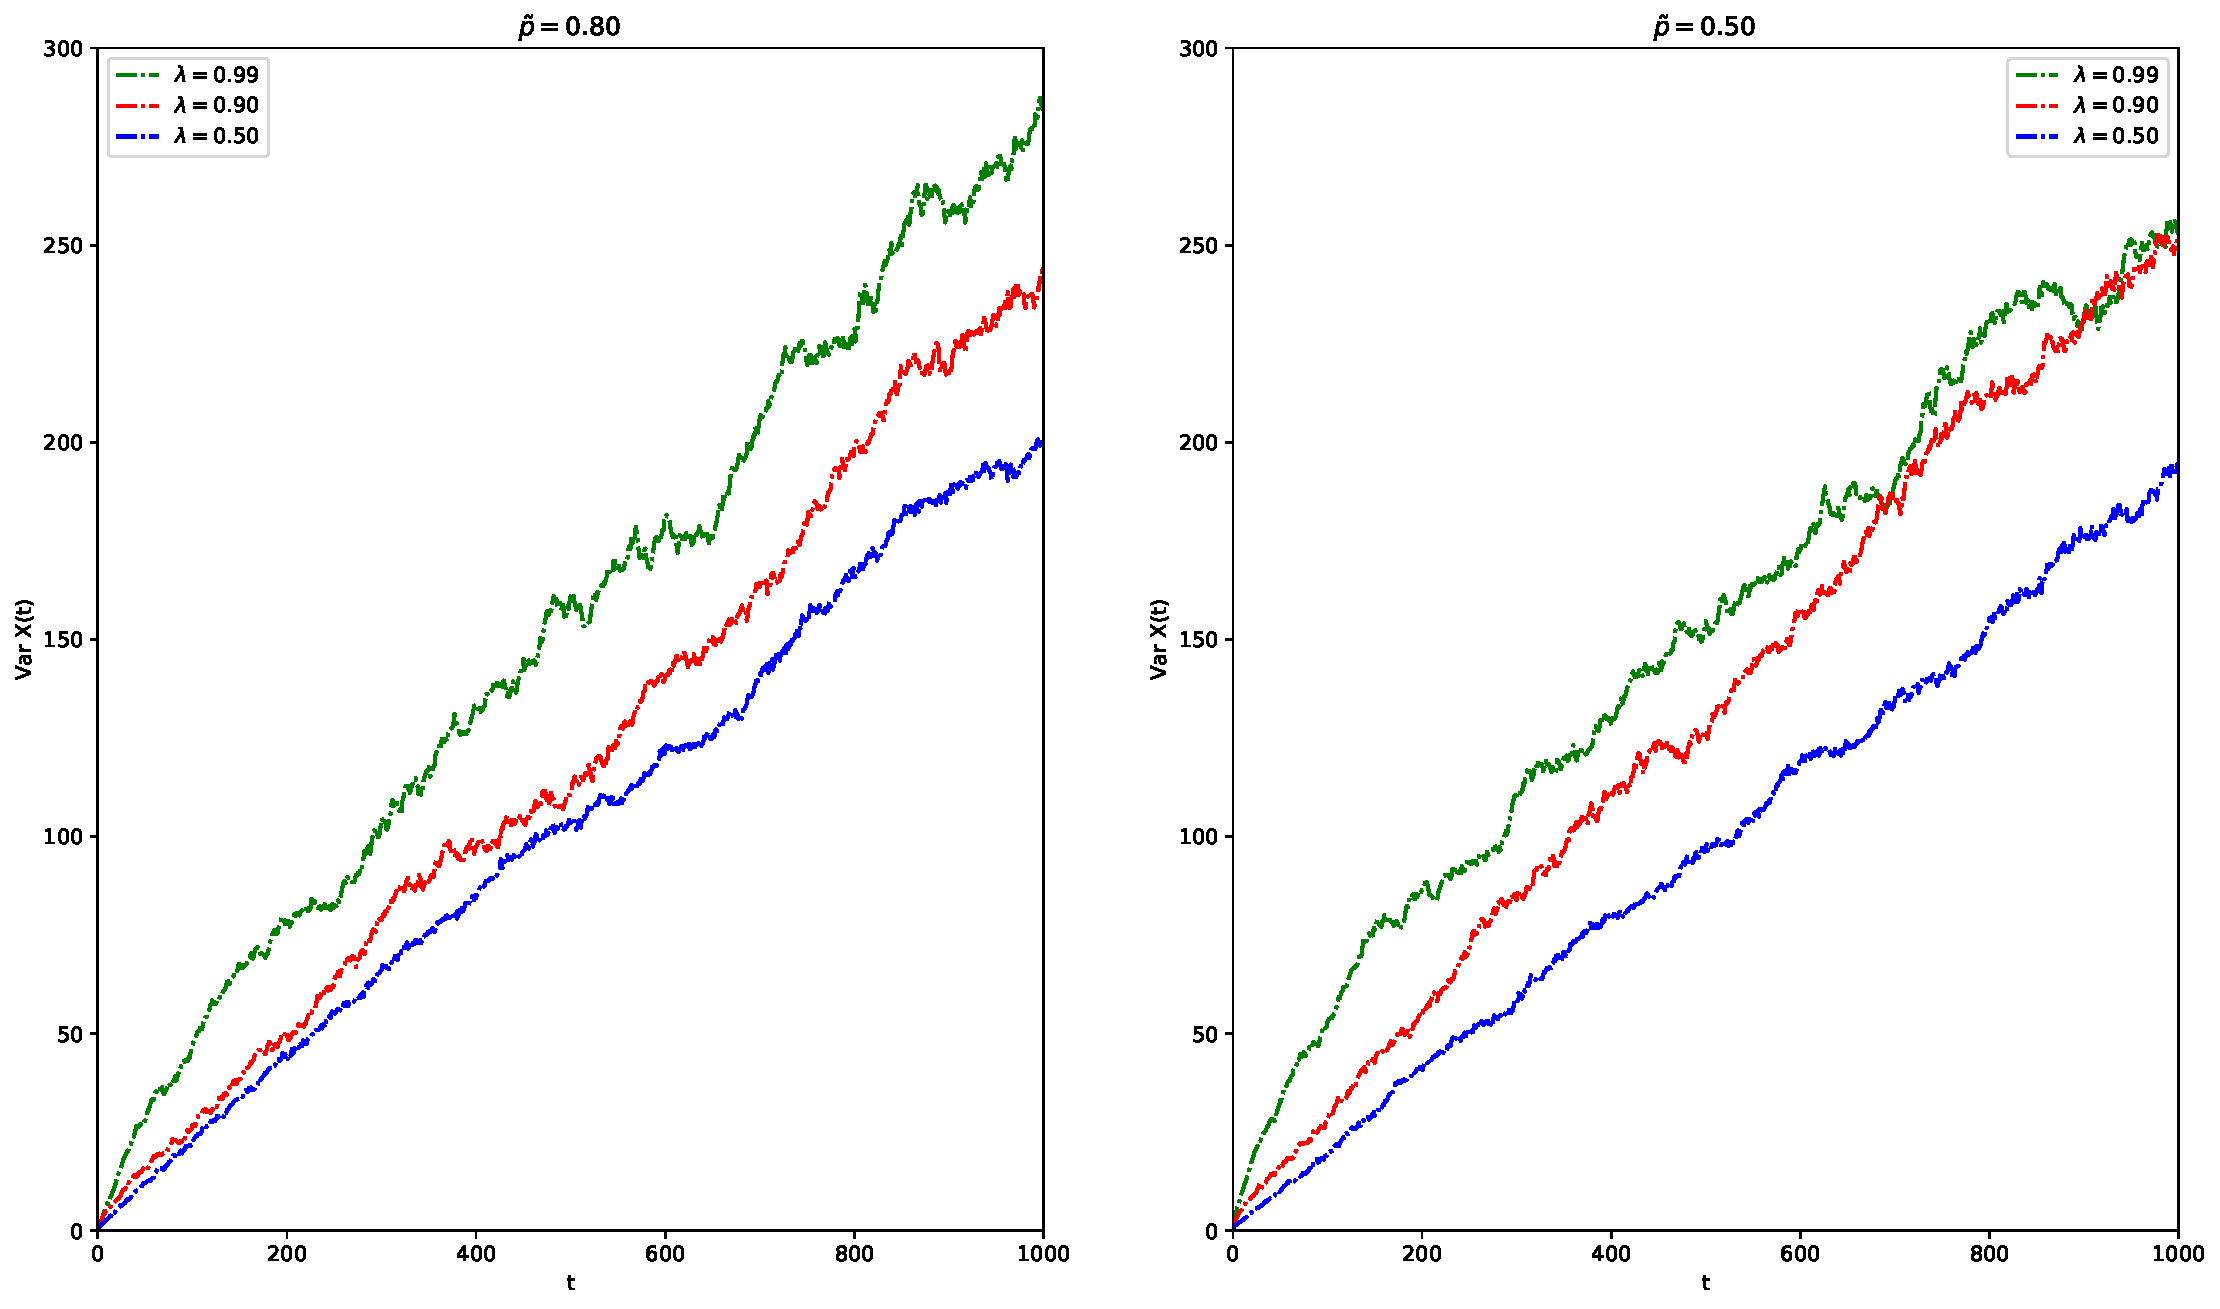
\includegraphics[width=1\textwidth]{VarXt}
\end{frame}
%
\begin{frame}{Alternative definitions}
\begin{itemize}
\item ``Success rewarded''
\[
X_{t-1}=1\rightarrow p_{t}=1-\lambda(1-p_{t-1})
\]
\[
X_{t-1}=0\rightarrow p_{t}=\lambda p_{t-1}
\]
\item Different coefficients for different events
\item Generally $n$ possible steps and $m$ different coefficients $\lambda$
affecting the transition probabilities
\item<0> Possible applications in
\begin{itemize}
\item<0> sports modeling
\item<0> reliability and survival analysis
\item<0> medical research
\end{itemize}
\item<0> Discrete alternative to random processes with memory
\end{itemize}
\end{frame}
%

\begin{frame}{Alternative definitions}

\end{frame}

%
\begin{frame}{Alternative definitions}
\begin{itemize}
\item ``Success rewarded''
\item Different coefficients for different events
\item Generally $n$ possible steps and $m$ different coefficients $\lambda$
affecting the transition probabilities
\[
p_{t}=f(p_{t-1},\,X_{t-1},\,\lambda_{1},\dots,\,\lambda_{m})
\]
\item<0> Possible applications in
\begin{itemize}
\item<0> sports modeling
\item<0> reliability and survival analysis
\item<0> medical research
\end{itemize}
\item<0> Discrete alternative to random processes with memory
\end{itemize}
\end{frame}
%
\begin{frame}{Alternative definitions}
\begin{itemize}
\item ``Success rewarded''
\item Different coefficients for different events
\item Generally $n$ possible steps and $m$ different coefficients $\lambda$
affecting the transition probabilities
\item<1-> Possible applications in
\begin{itemize}
\item<1-> sports modeling
\item<1-> reliability and survival analysis
\item<1-> medical research
\end{itemize}
\item<2-> Discrete alternative to random processes with memory
\end{itemize}
\end{frame}
%
\begin{frame}{RWWM Properties}
\begin{itemize}
\item tabulka 4x3 s vlastnostmi jednotlivych prochazek
\item Expected prob
\item Expected position
\item Expected variance
\item Comparision of the previous properties aplied for different model
types
\end{itemize}
\end{frame}
%
\begin{frame}{Asymptotic behaivor}

\begin{itemize}
\item Convergence to standard RW??
\item predchozi tabulka s hodnotami v nekonecnu
\end{itemize}
\end{frame}
%
\begin{frame}{Data generation}
\begin{itemize}
\item Ways to generate data, different conditions, number of repetitions
\item popis jaka data generuju
\end{itemize}
\end{frame}
%
\begin{frame}{Fitting on generated data}

\begin{itemize}
\item Which types are detectable and predictable from the data
\item Error rates
\item Grafy?
\end{itemize}
\end{frame}
%
\begin{frame}{Real life examples}

\begin{itemize}
\item Kratce popsat co jsem delal do Aten
\item Zminit, ze jsem desne vydelal na US Open
\end{itemize}
\end{frame}
%
\begin{frame}{Results}
\begin{itemize}
\item Zajimavy nastroj s possible implementations
\item link na github kam neco nahraju
\end{itemize}
\end{frame}
%
\begin{frame}{Next steps}
\begin{itemize}
\item Model implementation
\begin{itemize}
\item $\lambda$ optimization
\item $p_{1}$ optimization
\end{itemize}
\item<2-> Model improvement
\begin{itemize}
\item<2-> Other versions of random walk with memory
\item<2-> Combination with other approaches
\end{itemize}
\item<3-> Model testing
\begin{itemize}
\item<3-> Model evaluation granularity
\item<3-> Performance on a larger dataset
\item<3-> Bbetting module for more bookmakers
\item<3-> Application of the model to \emph{best-of-three} matches
\end{itemize}
\item<4-> Application in other domains
\end{itemize}
\end{frame}
%
\begin{frame}[plain] 
\begin{quote}%{} 
\begin{center} 
\huge{Thank you.} 
\end{center}
\vspace{10mm} 
\begin{center} 
\large{tomaskourim.com} 
\end{center}
\end{quote}%{} 
\end{frame}

\begin{frame}[plain] 
\begin{quote}%{} 
\begin{center} 
\huge{Thank you.} 
\end{center}
\vspace{10mm} 
\begin{center} 
\large{tom@skourim.com} 
\end{center}
\end{quote}%{} 
\end{frame}
\end{document}
